\section{Experimental results}

As many real-world datasets contain missing values, missing data imputation is an important problem in statistics and machine learning~\cite{little1986statistical, nelwamondo2007missing}.
Leveraging the structure underlying the data, GNNs have recently proved to be a powerful tool for this task~\cite{spinelli2020neural}.
Extending this view to higher-dimensional structure, we evaluate the performance of SNNs in imputing missing data over simplicial complexes.

\paragraph{Data.}
A \emph{coauthorship complex (CC)}~\cite{patania2017} is a simplicial complex where a paper with $k$ authors is represented by a $(k-1)$-simplex.
The added subsimplices of the $(k-1)$-simplex are interpreted as collaborations among subsets of authors---a natural hierarchical representation that would be missed by the hypergraph representation of papers as hyperedges between authors.
In general, a simplicial complex representing $n$-fold interactions (e.g.\ between authors) can be constructed as the one-mode projection of a multipartite graph (e.g.\ a paper-author bipartite graph).
The $(k-1)$-cochains are given by the number of citations attributed to the given collaborations of $k$ authors.
See Figure~\ref{fig:data2complex} and~\ref{fig:bipartite}, and the supplementary material for details.
We sampled (see the supplementary material) two coauthorship complexes---CC1 and CC2, see Table~\ref{table:Simplices-coauthor} for statistics---from the Semantic Scholar Open Research Corpus~\cite{ammar18NAACL}, a dataset of over $39$ million research papers with authors and citations.

\paragraph{Method.}
We evaluated the performance of the SNNs on the task of imputing missing citations on the $k$-cochains (for $k=0,1,2$) of the extracted coauthorship complexes.
As in a typical pipeline for this task~\cite{nelwamondo2007missing}, missing values are artificially introduced by replacing a portion of the values with a constant.
Specifically, given a fixed coauthorship complex, missing data is introduced at random on the $k$-cochains at $5$ rates: $10\%, 20\%,  30\% ,40\%$, and $50\%$.
The SNN is given as input the $k$-cochains on which missing citations are substituted by the median of known citations (as a reasonable first guess) and is trained to minimize the $L_1$ norm over known citations.
%\mdeff{Could be easier in math than text?}
We trained SNNs made of $3$ layers with $30$ convolutional filters of degree $N=5$ with Leaky ReLu for $1000$ iterations with the Adam optimizer and a learning rate of $10^{-3}$.

\paragraph{Results.}
Figure~\ref{fig:accuracy-error} shows the mean accuracy and absolute error distribution (see the supplementary material for definitions) of the SNN in inputing missing citations on CC1. Observe that the distribution of the prediction error accumulates close to zero.

\begin{figure}[htbp]
  \centering
  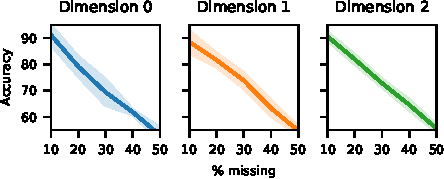
\includegraphics[height=2.7cm]{figures/performance_accuracy.pdf}
  \hfill
  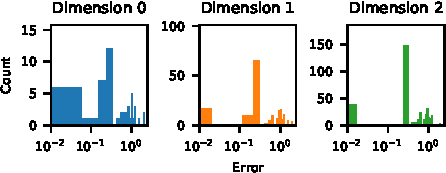
\includegraphics[height=2.7cm]{figures/performance_error.pdf}
  \caption{%
    Performance of SNNs.
    Left: Mean accuracy $\pm$ standard deviation over 5 samples in imputing missing citations on CC1.
    Right: Absolute error distribution over 1 sample for $40\%$ missing citations on CC1.
  }\label{fig:accuracy-error}
\end{figure}

%\paragraph{Baselines}
Table~\ref{tab:baselines} shows the performance of two baselines: missing values inferred as (i) the mean or median of all known values, and (ii) the mean of the $(k-1)$ and $(k+1)$ neighboring simplices.
SNNs well outperform these baselines.
Comparison with stronger imputation algorithms is left for future work.

%transfer/semi-supervized/transductive learning
To demonstrate that our filters transfer across complexes, we evaluated how accurately an SNN trained on one coauthorship complex can impute missing citations on a different complex.
We found that when imputing citations on CC1, a SNN trained on CC2 is almost as good as one trained on CC1 (compare Figures~\ref{fig:accuracy-error} and~\ref{fig:transfer-learning}).
We expect this result as coauthorship complexes share a similar structure, and the same process underlies the generation of citations across coauthorship complexes.
%same sample distribution (in train and test)

\begin{table}[htbp]
  \centering
  \begin{minipage}[b]{0.35\linewidth}
    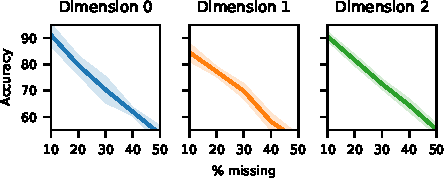
\includegraphics[width=\linewidth]{figures/performance_accuracy_transfer.pdf}
    \captionof{figure}{Performance on CC1 with an SNN trained on CC2.}\label{fig:transfer-learning}
  \end{minipage}
  \hspace{0.5cm}
  \begin{minipage}[b]{0.56\linewidth}
    \scriptsize{\begin{tabular}{lrrr}
      \toprule
      Method & Dimension 0 & Dimension 1 & Dimension 2 \\
      \midrule
      Global Mean & $3.30\pm0.82$ & $5.75\pm1.28$ & $2.96\pm0.49$ \\
      Global Median & $7.78\pm2.70$ & $10.44\pm1.00$ & $12.50\pm0.63$ \\
      Neighbors Mean & $11.88\pm5.29$ & $24.15\pm1.85$ & $27.38\pm1.18$ \\
      \bottomrule
    \end{tabular}}
    \vspace{9pt}
	\caption{Performance of baselines: mean accuracy $\pm$ standard deviation over 5 samples for $30\%$ missing citations on CC1.}\label{tab:baselines}
  \end{minipage}
\end{table}
